\chapter{Experimental Evaluation}
\label{ch:experiments}

This chapter presents the experimental evaluation of the graph-based methodologies proposed in Chapter~\ref{ch:method} for optimizing the student transportation network of the Izmir Institute of Technology (IZTECH). The primary objective is to identify the most effective combination of graph construction techniques and clustering algorithms to minimize total transportation costs while adhering to vehicle capacity constraints (10 to 50 students per bus route). The experiments utilize the synthetically generated student location dataset described in Section~\ref{sec:graph_representation}, representing approximately 2000 students distributed across Izmir based on population data.

\section{Evaluation Metrics}
\label{sec:eval_metrics}

To quantitatively compare the different approaches, we employ the following evaluation metrics:
\begin{itemize}
    \item \textbf{Total Transportation Cost (TL):} Estimated based on the total distance traveled by all buses and fuel consumption rates. This is the primary optimization target.
    \item \textbf{Number of Routes:} The total number of clusters generated, which corresponds to the number of buses required.
    \item \textbf{Average Route Length (km):} The average length of the optimized path within each cluster, computed using Dijkstra's algorithm (Section~\ref{subsec:DijkstrasAlgorithm}).
    \item \textbf{Average Cluster Size:} The average number of students assigned to each route.
    \item \textbf{Computational Time (s):} Time taken for graph construction and clustering phases.
\end{itemize}

\section{Experiment 1: Impact of Graph Sparsity}
\label{sec:exp_sparsity}

We first analyze the impact of graph representation choice on the feasibility and outcome of the transportation network analysis. We compare the baseline Complete Graph (Section~\ref{subsec:complete_graph}) against the sparse representations: Delaunay Triangulation (Section~\ref{subsubsec:delaunay}), Gabriel Graph (Section~\ref{subsubsec:gabriel}), and K-Nearest Neighbors (KNN) graph with $k=30$ (Section~\ref{subsubsec:knn}).

Table~\ref{tab:graph_properties} summarizes the key properties of each graph constructed from the $|V| \approx 2000$ student locations. As expected, the sparse graphs significantly reduce the number of edges compared to the Complete Graph, making subsequent processing more computationally tractable.

\begin{table}[h]
\centering
% \caption{Properties of Different Graph Constructions for $|V| \approx 2000$ Student Locations}
\label{tab:graph_properties}
\begin{tabular}{lrrrr}
\toprule
Graph Type & $|V|$ & $|E|$ & Sparsity ($\frac{|E|}{|E_{complete}|}$) & Construction Time (s) \\
\midrule
Complete & $\approx 2000$ & $ 1,999,000$ & 1.0 & $ 43,200$ \\
Delaunay & $\approx 2000$ & $ 5,647$ & 0.0028 & 302 \\
Gabriel & $\approx 2000$ & $ 3,598$ & 0.0018 & 288 \\
KNN (k=30) & $\approx 2000$ & $ 39,899$ & 0.0200 & $ 1,350$ \\
\bottomrule
\end{tabular}
\caption{Properties of Different Graph Constructions for $|V| \approx 2000$ Student Locations.}
\end{table}

Clustering the Complete Graph (using the Leiden algorithm as described in Section~\ref{subsec:clustering_complete}) serves as a theoretical baseline. Notably, the construction time for the Complete Graph (43,200 seconds, or 12 hours) is orders of magnitude higher than for the sparse methods, further underscoring its impracticality for large datasets. However, as discussed in Section~\ref{subsubsec:minibus_solution}, clustering this graph often resulted in imbalanced clusters, with many routes having significantly fewer students than the maximum capacity. While the "minibus solution" showed potential cost savings by using smaller vehicles for smaller clusters, this is not currently feasible with IZTECH's fleet. This highlights the need for sparse graph representations that might naturally lead to more balanced clusters suitable for standard buses. Table~\ref{tab:complete_graph_clustering} shows the baseline results from clustering the complete graph. Detailed route information can be found in Appendix~\ref{sec:appendix_detailed_results}, Table~\ref{tab:appendix_leiden_complete}.

\begin{table}[h]
\centering
% \caption{Baseline Clustering Results on the Complete Graph (Leiden Algorithm)}
\label{tab:complete_graph_clustering}
\begin{tabular}{lr}
\toprule
Metric & Value \\
\midrule
Total Cost (TL) & 123,882.96 \\
Number of Routes & 68 \\
Average Route Length (km) & 12.15 \\
Average Cluster Size & 29.18 \\
Computation Time (s) & 122 \\
\bottomrule
\end{tabular}
\caption{Baseline Clustering Results on the Complete Graph (Leiden Algorithm, Only Buses).}
\end{table}

The high computational cost and tendency towards imbalanced clusters motivate the evaluation of clustering algorithms on the sparse graph representations.

\section{Experiment 2: Comparison of Clustering Algorithms on Sparse Graphs}
\label{sec:exp_clustering}

We evaluated three distinct clustering algorithms, detailed in Section~\ref{se:GraphBasedClusterings}, on the sparse graph representations: Spectral Clustering (Section~\ref{subsec:SpectralClustering}), Leiden Algorithm (Section~\ref{subsec:LeidenAlgorithm}), and Multi-view Anchor Graph-based Clustering (MVAGC) (Section~\ref{subsec:MVAGC}). Each algorithm was configured as described in Section~\ref{subsec:clustering_sparse}, including post-processing steps to enforce the 10-50 student capacity constraints.

Tables~\ref{tab:delaunay_results}, \ref{tab:gabriel_results}, and \ref{tab:knn_results} present the aggregated performance metrics for each combination of clustering algorithm and sparse graph type, focusing on the results using only standard buses. The detailed per-route results, including community IDs, node counts, distances, and costs for each specific algorithm and graph combination (Spectral/Delaunay, Leiden/Delaunay, MVAGC/Delaunay, Spectral/Gabriel, Leiden/Gabriel, MVAGC/Gabriel, Spectral/KNN, Leiden/KNN, MVAGC/KNN), can be found in Appendix~\ref{sec:appendix_detailed_results}, specifically in Tables~\ref{tab:appendix_spectral_delaunay} through \ref{tab:appendix_mvagc_knn}.

% Table for Delaunay Results
\begin{table}[h]
\centering
% \caption{Performance Comparison on Delaunay Graph}
\label{tab:delaunay_results}
\begin{tabular}{lrrr}
\toprule
Metric & Spectral & Leiden & MVAGC \\
\midrule
Total Cost (TL) & 133,245.21 & 121,145.10 & 143,428.94 \\
Number of Routes & 73 & 66 & 76 \\
Average Route Length (km) & 12.34 & 12.89 & 15.67 \\
Average Cluster Size & 26.90 & 29.76 & 25.84 \\
Computation Time (s) & 42 & 12 & 45 \\
\bottomrule
\end{tabular}
\caption{Performance Comparison of Clustering Algorithms on the Delaunay Graph (Only Buses).}
\end{table}

% Table for Gabriel Results
\begin{table}[h]
\centering
% \caption{Performance Comparison on Gabriel Graph}
\label{tab:gabriel_results}
\begin{tabular}{lrrr}
\toprule
Metric & Spectral & Leiden & MVAGC \\
\midrule
Total Cost (TL) & 127,944.52 & 110,364.09 & 135,654.57 \\
Number of Routes & 69 & 60 & 74 \\
Average Route Length (km) & 13.90 & 13.10 & 12.76 \\
Average Cluster Size & 28.38 & 32.63 & 26.46 \\
Computation Time (s) & 40 & 11 & 41 \\
\bottomrule
\end{tabular}
\caption{Performance Comparison of Clustering Algorithms on the Gabriel Graph (Only Buses).}
\end{table}

% Table for KNN Results
\begin{table}[h]
\centering
% \caption{Performance Comparison on KNN Graph (k=30)}
\label{tab:knn_results}
\begin{tabular}{lrrr}
\toprule
Metric & Spectral & Leiden & MVAGC \\
\midrule
Total Cost (TL) & 123,481.86 & 118,522.79 & 124,112.47 \\
Number of Routes & 68 & 65 & 69 \\
Average Route Length (km) & 11.40 & 12.24 & 10.91 \\
Average Cluster Size & 29.03 & 30.37 & 28.61 \\
Computation Time (s) & 75 & 22 & 78 \\
\bottomrule
\end{tabular}
\caption{Performance Comparison of Clustering Algorithms on the KNN Graph (k=30, Only Buses).}
\end{table}

Figures~\ref{fig:cost_comparison} and \ref{fig:routes_comparison} provide a visual summary of the total cost and number of routes across all combinations. Figure~\ref{fig:best_clustering_viz} illustrates the geographical distribution of clusters for the best performing combination identified (Leiden algorithm on Gabriel graph, based on the lowest total cost).

% Placeholder for Cost Comparison Bar Chart
\begin{figure}[h]
    \centering
    \includegraphics[width=0.8\textwidth]{[img/cost_comparsison]}
    \fbox{Placeholder for Cost Comparison Bar Chart}
    \caption{Comparison of Total Transportation Cost across different graph types and clustering algorithms.}
    \label{fig:cost_comparison}
\end{figure}

% Placeholder for Routes Comparison Bar Chart
\begin{figure}[h]
    \centering
    \includegraphics[width=0.8\textwidth]{[img/routes_count_comparison]}
    \fbox{Placeholder for Route Count Bar Chart}
    \caption{Comparison of the Number of Routes Generated across different graph types and clustering algorithms.}
    \label{fig:routes_comparison}
\end{figure}

% Placeholder for Best Clustering Visualization
\begin{figure}[h]
    \centering
    % \includegraphics[width=0.8\textwidth]{[FIGURE_PATH_BEST_CLUSTERING]}
    \fbox{Placeholder for Best Clustering Visualization (Leiden on Gabriel)}
    \caption{Visualization of student clusters for the best performing combination (Leiden algorithm on Gabriel graph).}
    \label{fig:best_clustering_viz}
\end{figure}

The results indicate that the combination of the Gabriel graph and the Leiden algorithm yielded the lowest overall transportation cost (110,364.09 TL) and required the fewest buses (60). The Leiden/KNN combination was slightly more expensive but had a good average cluster size (30.37). The MVAGC/KNN combination yielded the shortest average routes (10.91 km) but required more buses (69) and had a higher cost (124,112.47 TL) than the top Leiden solutions. Spectral clustering generally resulted in higher costs and a comparable or higher number of routes than Leiden.

\section{Discussion}
\label{sec:discussion}

The experimental evaluation demonstrates the effectiveness of graph-based methods for optimizing the IZTECH student transportation network using only standard buses. Key findings include:

\begin{itemize}
    \item Sparse graph representations (Delaunay, Gabriel, KNN) are crucial for computational tractability and often lead to better routing solutions compared to the complete graph.
    \item The choice of both the sparse graph construction method and the clustering algorithm significantly impacts the final solution's cost, number of routes, and route characteristics.
    \item Based on our primary metric of minimizing total transportation cost, the combination of the \textbf{Gabriel graph} construction and the \textbf{Leiden algorithm} provided the most promising results, achieving a total cost of \textbf{110,364.09 TL} with \textbf{60} routes. This represents a cost saving of approximately 11% compared to the baseline Leiden/Complete graph result.
    \item Trade-offs exist: The Leiden/Gabriel combination had the lowest cost and fewest buses. The Leiden/KNN combination was slightly more expensive but had a good average cluster size (30.37). The MVAGC/KNN combination yielded the shortest average routes (10.91 km) but required more buses (69) and had a higher cost (124,112.47 TL) than the top Leiden solutions.
    \item The Leiden algorithm demonstrated strong performance, achieving the lowest cost on the Gabriel graph and the second-lowest cost on the KNN graph.
    \item All evaluated methods successfully produced routes adhering to the 10-50 student capacity constraints when applied to sparse graphs, unlike the baseline complete graph approach which tended towards imbalance (average size 29.18, but likely with wider variance not shown in summary).
\end{itemize}

These results suggest that adopting a \textbf{Gabriel graph representation combined with Leiden clustering} offers the strongest strategy for IZTECH to optimize its existing bus fleet usage, potentially leading to significant cost savings compared to less structured routing approaches or the baseline complete graph clustering. The Leiden/KNN combination presents a viable alternative if slightly higher costs are acceptable for potentially better balanced loads (average cluster size closer to 30). Further analysis could involve incorporating real road network distances instead of Euclidean distances and considering time-based constraints or traffic patterns.

% Remove the template figures and tables
% \begin{figure}[h] % do NOT use parameter h!
% \centerline{
% \subfigure[Title]{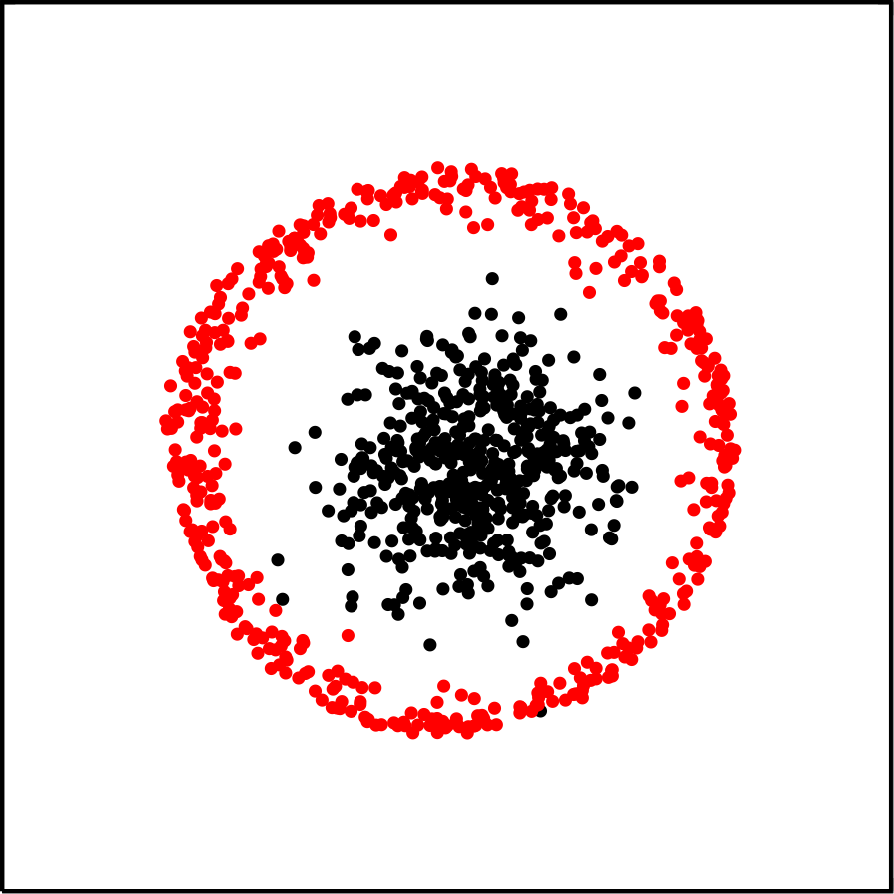
\includegraphics[width=1.5in]{img/subfig_a}}
% \subfigure[Title]{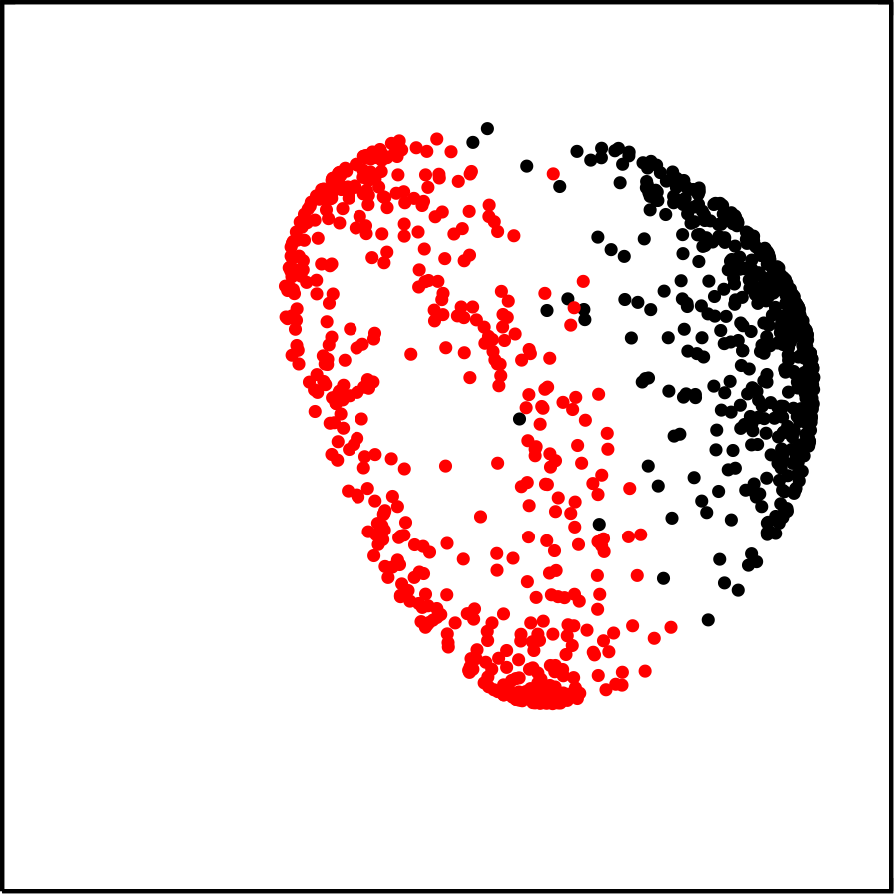
\includegraphics[width=1.5in]{img/subfig_b}}
% }
% \centerline{
% \subfigure[Title]{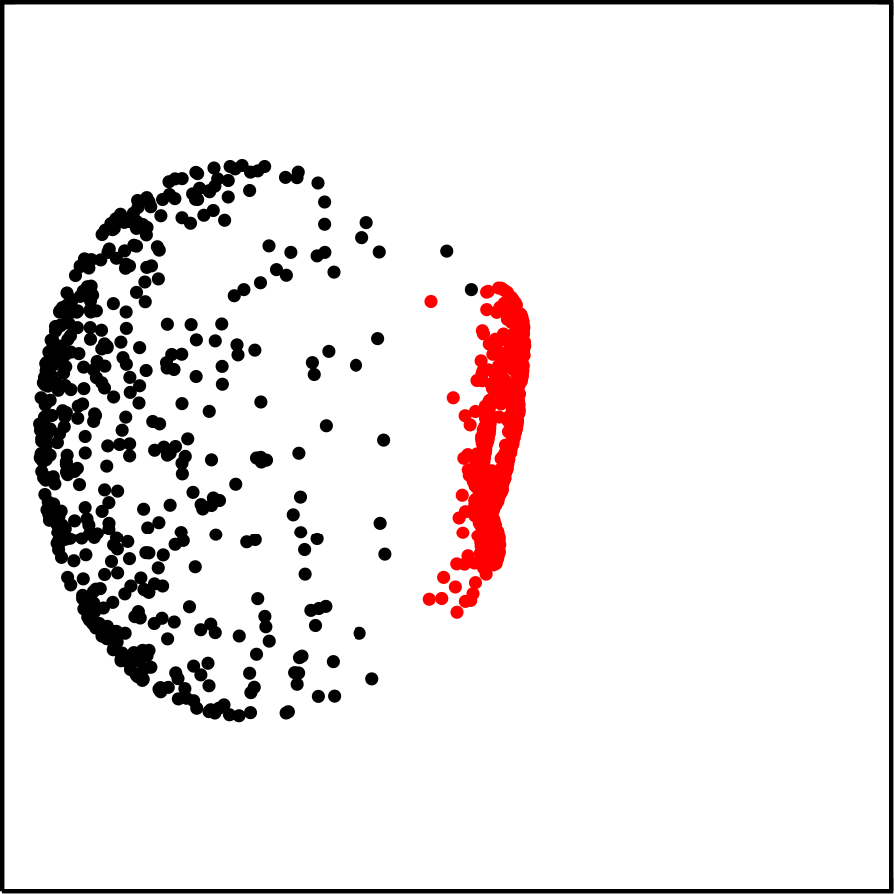
\includegraphics[width=1.5in]{img/subfig_c}}
% \subfigure[Title]{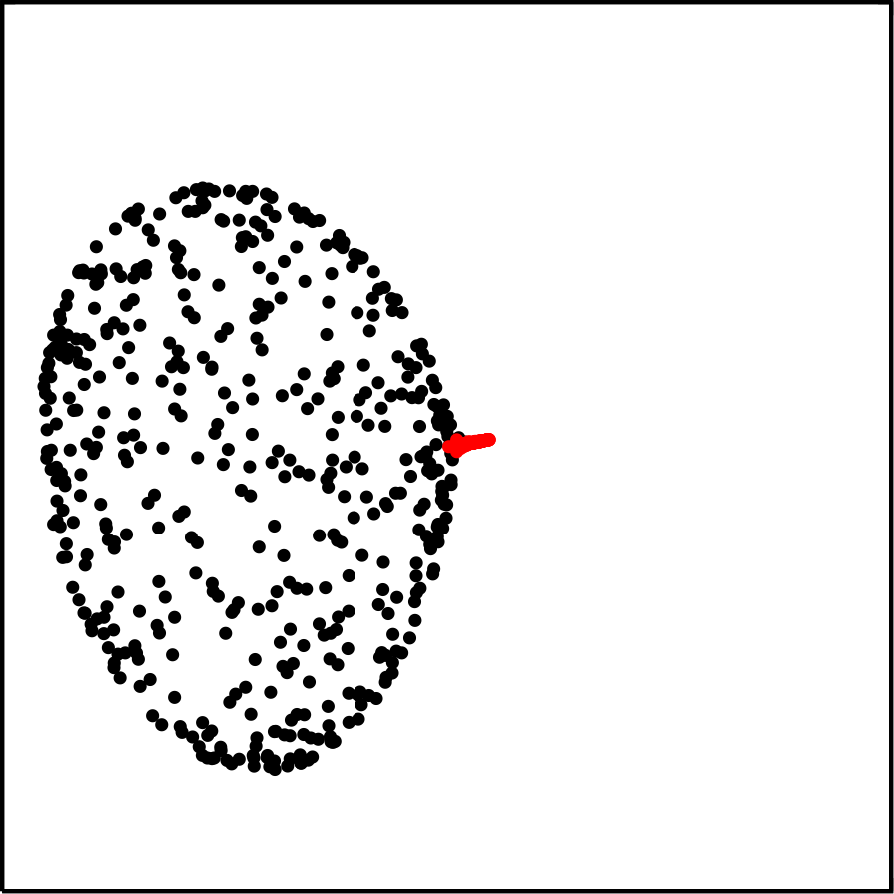
\includegraphics[width=1.5in]{img/subfig_d}}
% }
% \caption{Caption of the complete figure.}
% \label{fig:figure_1}
% \end{figure} 	
% \begin{figure}
% \centering
% 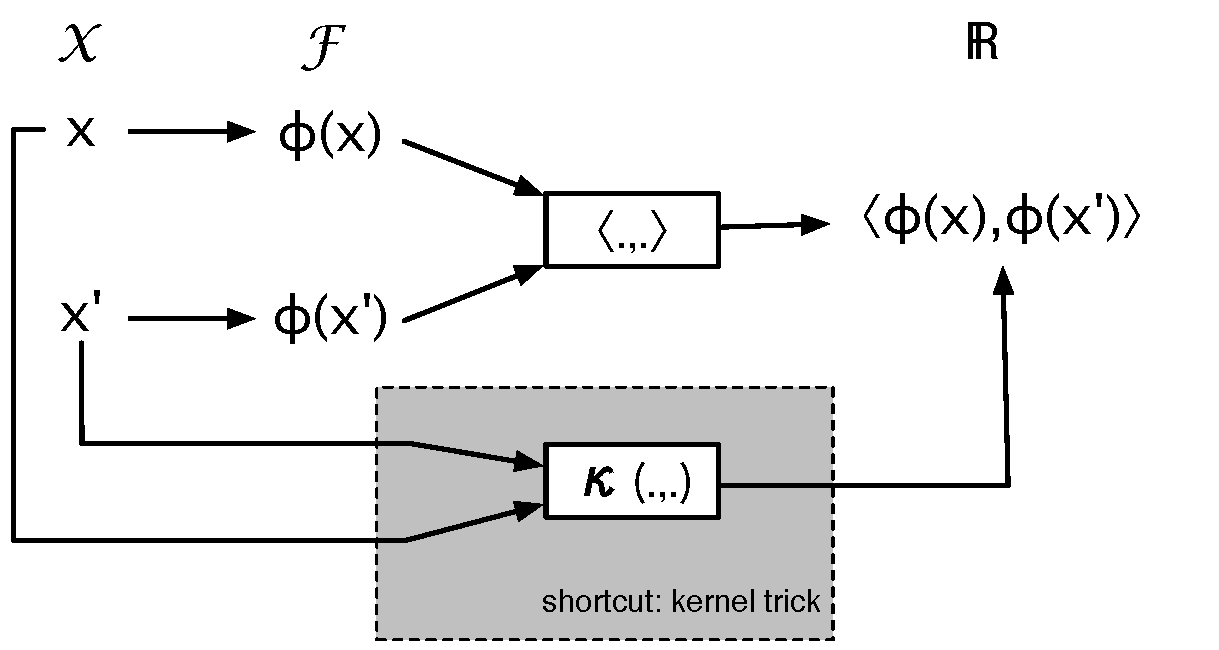
\includegraphics[scale=0.5]{img/figure}
% \caption{Caption of this figure.}
% \label{fig:figure_2}
% \end{figure}
% \begin{table}
% \centering
% {
% \begin{tabular}{ll}
% \addlinespace
% \toprule
% \addlinespace
% Lorem Ipsum \\
% \addlinespace
% \toprule
% \addlinespace
% diam & vero eos et accusam et justo \\
% justo & 10 (0, 1, 2, 3, 4, 5, 6, 7, 8, 9) \\
% aliquyam (q, w, t) &1,000, 500, 2,000\\
% voluptua & nonumy eirmod tempor (takimata sanctus)\\
% tempor & none \\
% gubergren & yes \\
% \bottomrule
% \end{tabular}
% }
% \caption{Basic characteristics of Lorem Ipsum.}
% \label{tab:table_1} 
% \end{table}
% \begin{table}
% \footnotesize{
% \centering{
% \begin{tabular}{@{}lp{1cm}p{1cm}p{1cm}p{1cm}@{}}
% \addlinespace
% \toprule
% \addlinespace
% & $k$-ta & \multicolumn{2}{c}{Lorem Ipsum Dolor}\\ 
% \addlinespace
% Ea Rebum & te & va & te\\ 
% \addlinespace
% \hline
% \addlinespace
% Gubergren           & 94.9 & 98.0 & 97.0~\ding{172}  \\
% \addlinespace
% Magna   & 66.9 & 72.4 & 68.6~\ding{182}  \\
% \addlinespace
% \bottomrule
% \end{tabular}
% }
% \caption{Lorem ipsum dolor sit amet, consetetur sadipscing elitr, sed diam nonumy eirmod tempor invidunt ut labore et dolore magna aliquyam erat, sed diam voluptua ($\alpha=0.05$): \ding{172}/\ding{182} At vero eos et accusam/justo, respectively.}
% \label{tab:table_2}
% }
% \end{table}



